\documentclass[titlepage,twocolumn]{article}
\usepackage{titlesec}
\usepackage[margin=.75in]{geometry}
\usepackage{graphicx,wrapfig}
\usepackage{multicol}
\usepackage{hyperref}
\usepackage{todonotes}
\usepackage{float}
\usepackage{csvsimple}
\usepackage{algorithm}
\usepackage{algorithmicx}
\usepackage[noend]{algpseudocode}
\usepackage{color,soul}
\graphicspath{{Images/}}
% \usepackage{thebibliography}

\newcommand{\HadoopEcosystem}{Hadoop Ecosystem}
\newcommand{\BigData}{Big Data}
\newcommand{\CityChicago}{City of Chicago}

\setlength{\columnsep}{.4 in}

\begin{titlepage}
\centering
\title{Analysis of Advertisement Data with Traffic Patterns Using The \HadoopEcosystem}
\author{Lawrence Gates \\ 
	{gateslm@rose-hulman.edu} \\ \\
	advised by Dr. Sriram Mohan \\ {mohan@rose-hulman.edu}
}
\end{titlepage}

\begin{document}
\maketitle
\onecolumn
\tableofcontents
\twocolumn

\begin{abstract}
	%\todo %{Find something to put here}
	The amount of data collected daily is rising. Various themes of data are collected for various reasons, such as temperature data, agricultural statistics, sales numbers, traffic data, and advertisement data. Using datasets, such as billboard advertisement data and congestion traffic, I have been able to effectively find areas of congestion for a given region or segment along with the best advertisement for the given region or segment. The \HadoopEcosystem\ environment was used in combination with the tools Apache Pig and Apache Hive. The traffic data was aggregated to find the statistics for a given region and segment on a given day. The randomly generated advertisement data was joined with each region and segment for a given day. For each of the days, a common time frame of overlap was found and was used to help determine if any congestion occurred in a given region and segment. To show the effectiveness of the algorithm, different time frames were used to show the impact of a certain advertisement in a given region and segment. 
\end{abstract}

\section{Motivation}

\par Many cities and states collect traffic statistics for roads, either to show traffic flow on display boards or to gather statistical information. This thesis serves as an example that any result can be used in other cities in order to attempt to record traffic data to find patterns and optimize advertisement locations. 
\par
Since the collection and storage of data has become easier with wireless sensors and the availability of cheaper storage, collecting traffic data within a well-funded location does not pose a problem. The only limitation is the sensors used to collect traffic data. Once a city has the data, providing data to the proposed algorithm should produce a result. With the creation of the algorithm, inputting traffic data should not be a hassle, and will provide useful marketing data for a city. 

\section{Theory and Concepts}

\par The essential points of this idea is using \BigData\ and a \BigData\ management system. The \BigData\ management system that is used is The \HadoopEcosystem. Additional details of The \HadoopEcosystem\ in respect to this thesis can be found in Section \ref{sec:hadoopEcosystem}.


\subsection{What is \BigData?}

\par \BigData\ is the ``Information asset characterized by such a High Volume, Velocity, and Variety to require specific Technology and Analytical Methods for its transformation into Value" \cite{doi:10.1108/LR-06-2015-0061}. The idea of \BigData\ is not limited to large companies, for instance, retailers trying to understand consumers shopping patterns, but also scientists performing analysis on data collected from experiments in a more timely manner. Based on the tool and environment used to master \BigData\ for a project, setting up and deploying the tool is not a simple task. Getting results from \BigData\ environment has the process of \cite{BigDataAndItsTechnicalChallenges}: 
\begin{enumerate}
	\item Acquisition
	\item Information extraction and cleaning
	\item Data integration
	\item Modeling and analysis
	\item Interpretation and deployment
\end{enumerate}

\par \BigData\ is not guaranteed to produce a result with any given dataset. Data is not guaranteed to produce a pattern. A success from \BigData\ can come from showing a pattern or trend within a given dataset or by finding a lack of trend in a large amount of data. By using a \BigData\ environment or tools, analysis of the data can produce a result based on what the user designs for the modeling and analysis stage as well as the interpretation and deployment stage, not just running the data through the tool itself. 


\section{Literature Review}% \todo{ Be Assertive}}

Currently, there has been no academic research into using \BigData\ and coordinating traffic flow with advertisements. However, there has been plenty of academic research and articles involving \BigData\ and traffic datasets, along with many articles about the applications of using \BigData\ and advertisements.
\par
Smith and Demetsky \cite{smith1997traffic} discussed the importance of “intelligent transportation systems,” at a time before Google Maps and traffic flows were available on the internet. Their paper discusses the need to have forecasting models, using several time prediction techniques, such as machine learning and historical average, to determine traffic forecasting. With the datasets being collected, this project is using historical averaging with the available data. Daas, Puts, Buelens, and van den Hurk \cite{BigDataOfficialStats} highlight that, at the time, \BigData\ was heavily viewed from an “IT-perspective” and “focus[ed] on soft[ware] and hardware issues.” In the \BigData\ case study done by Chen, Pao, and Lee \cite{7004425} about the study of traffic loop detection data, a successful plot of peak hours and vehicle flow was shown. The case study shows the high potential of finding a trend in traffic data.
\par
The \BigData\ and advertisement side of academic articles talked about the collection and use of user data. Couldry and Turow \cite{IJoC2166} elaborate on personalized advertising constantly mining personalized data. The article also looks “more broadly at the consequences of embedding \BigData\ use in advertising,” which is not of concern for this thesis. Bughin, Chui, and Manyika \cite{7bac15dae50148d98f3263d7f91d8130} discuss the opportunities companies take with using the data available for a web-based company. The availability of data for marketing is not scarce due to the expanding amount of data, which is to be useful in determining advertisements to display in a certain area.
								
\section{Data and Operationalization}

To successfully complete the thesis, a vast amount of traffic data was needed and advertisement data to show a relationship between the two datasets as well as show the different types of analysis compared against each other and the varying results that were available. 

\subsection{Data}
\label{sub:Data}

\par The \textit{Chicago Data Portal} is the preferred mechanism to share all the data that is collected throughout The \CityChicago\ daily. The \textit{Chicago Data Portal} was established through the \href{https://www.cityofchicago.org/city/en/narr/foia/open_data_executiveorder.html}{Open Data Executive Order (No. 2012-2)} to add a level of transparency to the data being collected by Chicago officials. 

\par The data that is essential for determining traffic flow within Chicago are the
\href{https://data.cityofchicago.org/Transportation/Chicago-Traffic-Tracker-Congestion-Estimates-by-Se/n4j6-wkkf}{Chicago Traffic Tracker - Congestion Estimates by Segment} and the  \href{https://data.cityofchicago.org/Transportation/Chicago-Traffic-Tracker-Congestion-Estimates-by-Re/t2qc-9pjd}{Chicago Traffic Tracker - Congestion Estimates by Regions} datasets. Please refer to Appendix \ref{app:segmentCTT} and \ref{app:regionCTT} for information about the downloaded spreadsheets.

\subsubsection{Chicago Traffic Tracker - Congestion Estimates by Segments}

\par The segment estimations “contains the current estimated vehicle speed for about 1250 segments covering 200 miles of arterial roads” \cite{S1} in Chicago. The spreadsheet does not update every segment, which is due to an uploading problem on the data portal`s end. The segment estimations are roughly collected every 20 minutes by the Data Portal. The important information from each row in the dataset are:
\begin{enumerate}
	\item Location of the traffic flow
	\item Area of the traffic flow
	\item Speed of the traffic
	\item Time stamp the data was updated
\end{enumerate}

\par Since the segments are sub-areas of a region, more options for finding optimal advertisement placement will be available, compared to having only 29 regions to find optimal advertisement placement. Refer to the Appendix \ref{app:segmentCTT} for information about the columns of the dataset. Data was collected between September 18th, 2016 to February 23rd, 2017. Details of the automatic download is shown in Algorithm \ref{alg:1} and in the repository in Section \ref{sub:github} under the \textit{Scripts/automatedRun.sh} file.

\par The algorithm starts by getting the previous region and segment files from the local directories. The current date time is retrieved and the files appropriate file names for region and segment are initialized with the current date time. The new region and segment files are downloaded from The \CityChicago\ Data Portal. Downloading the \textit{csv}, \textit{json}, and \textit{xml} for each segment, each of these files are stored in the appropriate region and segment directory. The new files are compared to the previous files, checking if the contents are the same. If the contents of each set of files are the same, the new files with the same content are deleted. After the counter of 60 minutes, an email is sent with a status update. 

\begin{algorithm}
	\small
	\caption{\small Automated Download from The \CityChicago\ Data Portal}
	\label{alg:1}
	\begin{algorithmic}[1]
		\Procedure{main}{}
		\State $regPrevF \gets ``"$
		\State $segPrevF \gets ``"$
		\While{$true$}
		\State $regPrevF \gets \Call{GetPrevRegFile}{}$
		\State $segPrevF \gets \Call{GetPrevSegFile}{}$
		\State $dateTimeNow \gets \Call{GetSysTime}{}$
		\State $regFileNm \gets ``regEst-"\$dateTimeNow$
		\State $segFileNm \gets ``segEst-"\$dateTimeNow$
		\State \Call{DownloadToFiles}{regFileNm, segFileName}
		\If {$\Call{cmp}{regPrevF, regFileNm} \neq SAME$}
		\State $\Call{RemoveNewFile}{regFileNm}$
		\EndIf
		\If {$\Call{cmp}{segPrevF, segFileNm} \neq SAME$}
		\State $\Call{RemoveNewFile}{segFileNm}$
		\EndIf
		
		\State $\Call{sleep}{5m}$
		
		\State $counter \gets counter + 5$
		
		\If{$counter < 60$}
		\State $DATE = \Call{GetSystemTime}{}$
		\State $counter \gets 0$
		\State $Send Status Update via Email$
		\EndIf
		
		\EndWhile
		
		\EndProcedure
	\end{algorithmic}
\end{algorithm}

\subsubsection{Chicago Traffic Tracker - Congestion Estimates by Regions}

\par The region estimations “contains the current estimated congestion for the 29 traffic regions” \cite{S3} in Chicago. The region spreadsheet stored on the \textit{Chicago Data Portal} has updated all 29 regions. The region estimations are to be collected every 10 minutes by the Data Portal. The important information from each row in the dataset are the boundary of a given region, speed of the traffic, and the time stamp the data was updated. Since the 29 regions each have a given number of segments, a given region will provide an overview of the average speed of all the segments. By having segments in each region, a pattern can be found about the given region. This can be used to find the best advertisement over the region, then finding a better fit of the advertisement in a smaller defined area, such as a segment. Refer to Appendix \ref{app:regionCTT} for information about the columns of the dataset. Data was collected between September 18th, 2016 to February 23rd, 2017. Details of the automatic download is demonstrated in Algorithm \ref{alg:1} and in the repository \ref{sub:github} under the \textit{Scripts/automatedRun.sh} file. The downloading of regions datasets operations happen with the downloading of the segment datasets.

\subsection{Advertisement Data}
\label{sub:adData}

\par Due to the confidentiality and cost of purchasing advertisement data, using accurate data gathered by companies was not available for the scope of the thesis. The type of a billboard advertisement that was successful in a given area and the length of time the advertisement that was left on the billboard was needed in order to find a trend in traffic congestion and advertisement. To overcome this set back, advertisement data was randomly generated for each region and segment to represent an advertisement for the region and segment itself for a given time frame. The data manually generated randomly assigns an advertisement theme from Appendix \ref{app:adThemes}. A theme for a given region will last from a single day up to 30 days, which would have a theme randomly assigned for a new given time period. 
\par Details of the random advertisement generation for every segment and region is shown in Algorithm \ref{alg:2} and in the repository \ref{sub:github} under the subproject \textit{Projects/GenerateThoroughBillboardData}. The algorithm loops through all the segments and regions, starting with the first date of the traffic data. While looping through the days, a random rating for the theme is assigned from the list of advertisement themes, a random rating of success for the advertisement theme, and a random length of time for the advertisement theme to stay active, from 1 day to 30 days. The random advertisement theme and rating stays the same for the length of the random time length while the day increments. Once the length of the random time is completed, a new random theme, rating, and time length is assigned. This process continued until the last day of data collection. 

\begin{algorithm}
	\small
	\caption{\small Randomly generate advertisement data for segments and region.}
	\label{alg:2}
	\begin{algorithmic}[1]
		\Procedure{main}{}
		\State $segmentFIle \gets\Call{generateSegmentData}{}$
		\State $ regionFile \gets \Call{generateRegionData}{} $
		
		\EndProcedure
		\Procedure{generateSegmentData}{}
		\For{$s:=1\textbf{ To } 1310 $}
		\State $ curDt \gets startDate $
		\While{$ curDt \textbf{ BEFORE } endDate$}
			\State{$ adThm \gets \Call{Rand}{AD\_THM\_COUNT} $}
			\State{$ r \gets \Call{Rand}{MAX\_RATING} $}
			\State{$ ad\_len \gets \Call{Rand}{AD\_LEN} $}
			\For{$ date:=1 \textbf{ TO } ad\_len $}
				\State{$ curSeg \gets SegMdl(s,curDt,adThm,r)$}
				\State{$ curDt \gets curDt + 1 $}
				\State{$ segAds[\ ] \gets curSeg$}
			\EndFor
		\EndWhile
		\EndFor
		\Return{$segAds$}
		\EndProcedure
		\Procedure{generateRegionData}{}
		\For{$rN:=1\textbf{ To } 29 $}
		\State $ rg \gets REGION\_NAMES[rN] $
		\State $ curDt \gets startDate $
		\While{$ curDt \textbf{ BEFORE } endDate$}
		\State{$ adThm \gets \Call{Rand}{AD\_THM\_COUNT} $}
		\State{$ r \gets \Call{Rand}{MAX\_RATING} $}
		\State{$ ad\_len \gets \Call{Rand}{AD\_LEN} $}
		\For{$ date:=1 \textbf{ TO } ad\_len $}
		\State{$ curReg \gets RegMdl(rg,curDt,adThm,r)$}
		\State{$ curDt \gets curDt + 1 $}
		\State{$ regAds[\ ] \gets curReg$}
		\EndFor
		\EndWhile
		\EndFor
		\Return{$regAds$}
		\EndProcedure
	\end{algorithmic}
\end{algorithm}

\subsection{Census Data}
\label{sub:censusData}

\par To overcome the lack of advertisement targeting data, census data could be used as a substitute. Census data gathered by the United States contains many statistics to determine factors of a given area, with such statistics as: age, education, housing, income, poverty, race, and veterans. Users can find data based on a state, county, city, town, or zipcode, available on the \href{https://www.census.gov/}{United States Census Bureau}. The \CityChicago\ is comprised of \href{http://zipcode.org/city/IL/CHICAGO}{85 zipcodes}, but the number of zipcodes all the regions overlap is 74 zipcodes, displayed in the Figure \ref{fig:RegionZipCodeMap}.

\begin{figure}[H]
%\onecolumn

\centering
\includegraphics[scale=.45]{RegionZipCodeOverLay.png}
\caption{\small Map of Chicago overlayed with the zipcode (gray) and the North-East corner and South-West corner matching in color for all 29 region}
\label{fig:RegionZipCodeMap}
\end{figure}
%\twocolumn

To use zip codes for the census data is a large task in itself. A region or segment was not bounded by a given zip code, which allowed overlap for zip codes within a region. To determine the amount a given zip code overlays inside a region would require a significant amount of mathematics and accurate geographical data to ensure that the area of a zip code was factored in correctly to a region. The amount of work was beyond the scope of the thesis, described in \hyperref[sec:futureWork]{Future Work}

\par In the repository \ref{sub:github}, a subproject called \textit{Projects/DataCollection} used a library called \emph{\href{https://jsoup.org/}{jsoup}}. \emph{jsoup} is used to parse real-world HTML. The project takes the URLs of census data for given zipcodes and extracts data from HTML tables to CSV readable files. The data downloaded is essential for incorporating census data to zipcodes without finding or paying for easily accessible datasets.  

\par The \emph{jsoup} tool is designed for Java, allowing for easy extraction of data. To extra census data from a zipcodes, the general layout of a given site needs to be understood. Following the HTML on the site, a general flow is located and \emph{jsoup} can walk the HTML tree and pull out the HTML element nodes. Once the specific nodes are collected, the data can be stored separately from the HTML and then placed all together in a spreadsheet for easy reading and analysis. 

\subsection{\HadoopEcosystem}
\label{sec:hadoopEcosystem}

\par The \HadoopEcosystem\ was created by \href{http://hadoop.apache.org/}{Doug Cutting}, who created \href{http://lucene.apache.org/}{Apache Lucene}. Hadoop takes advantage of using a distributed file system, the Hadoop Distributed File System (HDFS), to handle storage needs of large files that need to be browsed. To handle large jobs, a MapReduce implementation was created to accomplish the job in The \HadoopEcosystem\ \cite{white_2015:Ch1}. % Chapter 1

\subsubsection{Hadoop Distributed File System}

Datasets have the potential to be larger than the storage of a single computer, resulting in breaking the data apart to store on multiple computers. The multiple computers are not required to have expensive hardware, but rather can be commodity computers. The computers, each a node in the cluster, are designed to store and pass data between each other and perform jobs on the node itself. An additional feature of HDFS is handling very large files, that can be split up across multiple nodes in a server, allowing for easy access to specific parts of file for processing. The streaming of data across the nodes is essential to follow the most efficient data processing pattern, ``write-one, read-many-times pattern" \cite{white_2015:Ch2Pg44}, to allow a dataset to be copied from the originating node and have various operations performed on the whole or portions of the dataset over time \cite{white_2015:Ch2}. % Chapter 2

\subsubsection{MapReduce}

MapReduce jobs are specifically designed for large dataset problems by splitting up the data to be run in parallel. In The \HadoopEcosystem, the job submitted on data is separated into two different tasks: map tasks and reduce tasks. The map task takes the data and applies a filter and will sort the data into a desired output based on parameters and store the mapped result back to disk, to avoid replicating an intermediate value. The mapped results will then be processed through a reducer, where an operation is performed, such as aggregation, among the filtered data. In figure \ref{fig:mapReduceDiagram}, multiple maps of data being split are being pushed into the reduce function to get an output based on some sort of user-defined function. 

\begin{figure}[H]
	%\onecolumn
	\centering
	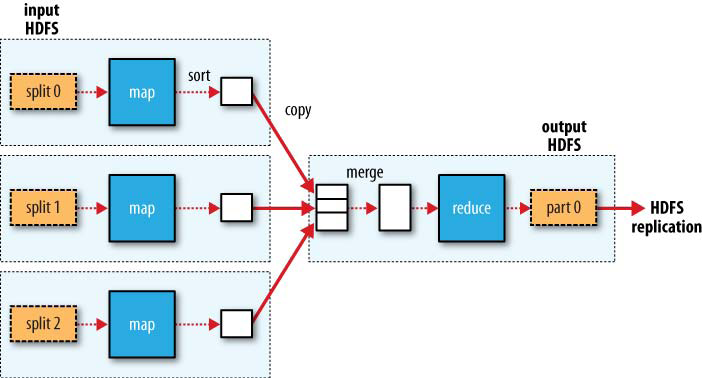
\includegraphics[scale=.35]{mapReduceDiagram.png}
	\caption{\small MapReduce data flow with a single reduce task \cite{fei_2011}}
	\label{fig:mapReduceDiagram}
\end{figure}

\subsection{The \HadoopEcosystem\ Tools}

The \HadoopEcosystem\ has a library of predefined projects that can be incorporated into the ecosystem. These projects often provide a high level language to process data in a manner similar to native MapReduce operations but allowing a user to forgo the requirement of making such a MapReduce program. Tools can be language-neutral data serialization systems, storage format systems, extracting data from structured data stores, and MapReduce abstraction. All these available tools can be used along side a user-defined  MapReduce function.  

\subsubsection{Apache Pig}

Apache Pig allows users to take MapReduce jobs to a higher level of abstractions when processing datasets. Compared to a MapReduce job, the time required to construct a Pig script to process data is extremely shorter and much more straightforward. Many operations that are supported by Pig are not ideal in MapReduce jobs, such as handling a join of data. Data can be passed into Pig to allow for cleaning, removing columns from spreadsheet datasets, or removing rows that have data that does not match a type or is a certain value \cite{white_2015:Ch16}. 

\subsubsection{Apache Hive}

%\HadoopEcosystem itself is not a database management system, but data can potential stored after processing in such a format that would be ideal to be accessed in a database management system. 
Apache Hive is a data warehouse framework that utilizes the way data is stored in HDFS and accesses such data in SQL type format. Hive handles processing a query on a large number of datasets stored in HDFS, allowing for the creation of tables, joining results together easily, and aggregating results for additional processing \cite{white_2015:Ch17}. 


\section{Architecture}


\par Due to the large amount data stored within the dataset, an architecture flow was needed to do a complete analysis of the data and combined with advertisement data. The data flow of the cluster pulls in \textit{Congestion Estimates by Segment} and \textit{Congestion Estimates by Region} from the Chicago Data Portal. Three files are downloaded, as back-up copies in alternative forms, as visualized in Figure \ref{fig:DataDownload}. 

\begin{figure}[h]
	\centering
	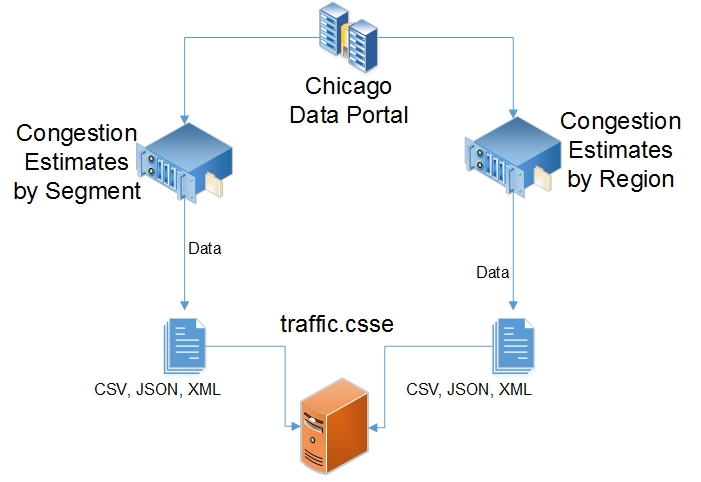
\includegraphics[scale=.4]{DataStorageDrawing.jpg}
	\caption{\small Dataflow of downloading data from the Chicago Data Portal.}
	\label{fig:DataDownload}
\end{figure}

\par Using an available API, data is downloaded directly to a node used primarily for initial storage and alerting status of files download. The details of the download are mention in Algorithm \ref{alg:1}. Since the data is stored remotely from the Hadoop cluster, the specific file format, \textit{csv}, that is used is transferred to the cluster, leaving data that is not used off the cluster, \textit{xml} and \textit{json}. 

\par The spreadsheet files for regions and segments are transferred to the cluster and stored in HDFS. Once on the cluster, the traffic data for regions and segments are cleaned and processed separately. The region traffic data has the the region name, speed and date time for each row of every region spreadsheet stored in the folder matching the day the data was collected. 


\begin{figure}[ht]
	\centering
	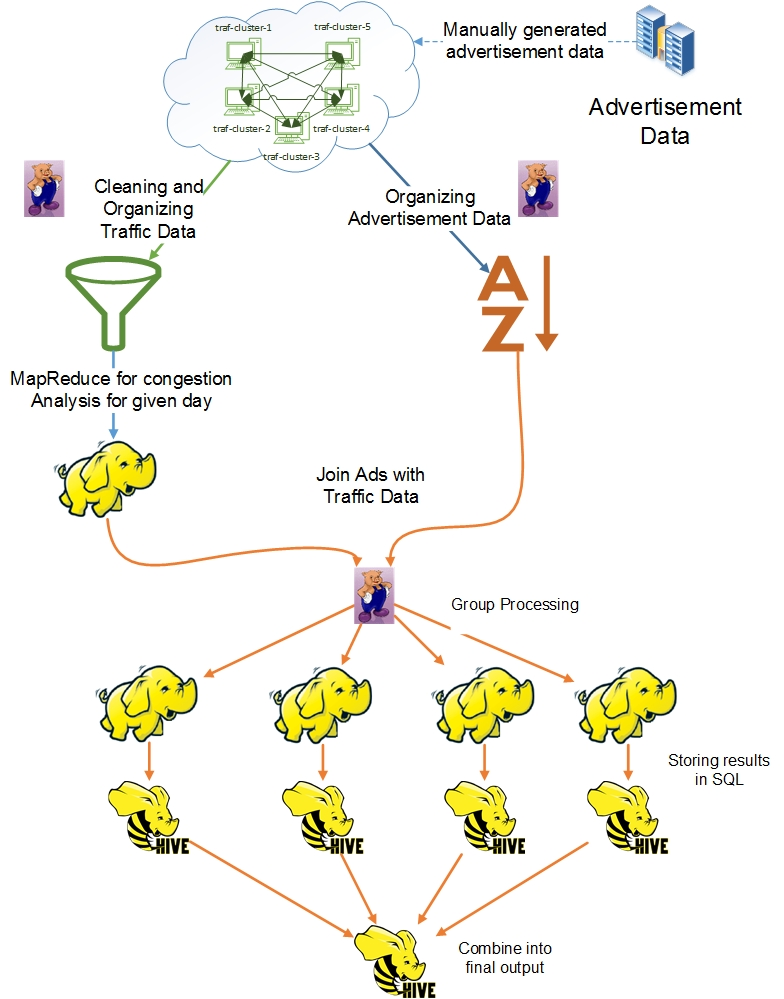
\includegraphics[scale=.45]{FinalCleaningAndProcessing.jpg}
	\caption{\small Dataflow for processing the traffic and advertisement data}
	\label{fig:DataProcessing}
\end{figure}

\par The data stored in the cluster can  be retrieved, which is then passed to The \HadoopEcosystem\ with various aggregation and analysis done on the given data, visualized in Figure \ref{fig:DataProcessing}. The region and segment traffic data is cleaned and processed in a similar format, storing the region name and segment id, speed and date time for each row of every region and segment spreadsheet stored in the folder matching the day the data was collected. For each day of every region and segment, the traffic data is calculated to form sums of specific congestion classifications. Using the descriptions from the Chicago Data Portal, the speeds are used to classify the type of congestion. 

\par The advertisement data is stored in HDFS, which is processed by a Pig script. The Pig script separates the advertisement data by segment and region, then storing the advertisement ratings for a given segment and region into separate folders. The advertisement data requires less cleaning and aggregation initially, as compared to the region and segment data. The advertisement data is randomly generated, thereby avoiding noise, removing the need for such cleaning. 

\par The advertisement data is joined with the region and segment traffic data, as shown in the middle of Figure \ref{fig:DataProcessing}. After combining the data two different datasets, forming region and segment traffic advertisement. Each one of the theme sets are processed through the MapReduce jobs, separated into four types of date grouping. The data is either all grouped together, by week of a year, month of a year, or by year. Each one of the groupings is then exported to a Hive table allowing for the aggregating of the highest for each region and segment individually, based on the grouping of the date, and stored into a final result. 

\section{Algorithms}
\label{sec:algorithms}

\par Pig and Hive help aggregate the data, however a more unique user-defined function is needed at continue process. To handle the classification of congestion for each date time, the speed is collected and the data is aggregated to find the best advertisement for that region or segment.

\subsection{Advertisement Storage}

\par The data is easily transferred from the initial spreadsheet file to a formatted file on the cluster. This operation was done with a Pig script for both the segment and region advertisement data. An example dataset is shown in Figure \ref{tab:regionAdsTable}. The segment advertisement data looks very similar, except the first column is \textit{Segment ID}, rather than \textit{Region Name}. 

% Table generated by Excel2LaTeX from sheet 'regionAds'
\begin{figure}[h]
	\centering
	\footnotesize
	\begin{tabular}{|l|l|l|r|}
		\hline
		Region Name & Date & Theme & Rating \\
		\hline
		Near South-Douglas & 2017-13-2 & Religious & 5 \\
		Near South-Douglas & 2017-14-2 & Religious & 5 \\
		Near South-Douglas & 2017-15-2 & Religious & 5 \\
		Near South-Douglas & 2017-16-2 & Religious & 5 \\
		Near South-Douglas & 2017-17-2 & Religious & 5 \\
		Near South-Douglas & 2017-18-2 & Religious & 5 \\
		Near South-Douglas & 2017-19-2 & Religious & 5 \\
		Near South-Douglas & 2017-20-2 & Restaurant & 7 \\
		Near South-Douglas & 2017-21-2 & Restaurant & 7 \\
		Near South-Douglas & 2017-22-2 & Restaurant & 7 \\
		Near South-Douglas & 2017-23-2 & Restaurant & 7 \\
		South West Side & 2016-18-9 & Theater & 1 \\
		South West Side & 2016-19-9 & Theater & 1 \\
		South West Side & 2016-20-9 & Theater & 1 \\
		South West Side & 2016-21-9 & Theater & 1 \\
		South West Side & 2016-22-9 & Theater & 1 \\
		South West Side & 2016-23-9 & Theater & 1 \\
		South West Side & 2016-24-9 & Theater & 1 \\
		\hline
	\end{tabular}%
	\label{tab:regionAdsTable}%
	\caption{\small Subset of data from region advertisement data that was randomly generated by Algorithm \ref{alg:2}. The algorithm that controls the generation fo random advertisement data is shown in Section \ref{sub:adData}}
\end{figure}%


\subsection{Traffic Analysis}

\par Once the traffic data is downloaded, it needs to be cleaned and sorted. Then traffic data and the advertisement data need to be integrated together. To successfully process the traffic data and combine with the advertisement data, two different algorithms are needed. 

\subsubsection{Cleansing Data}

\par The data obtained from The \CityChicago\ Data Portal is not set up to be directly integrated into the analysis algorithms, requiring the datasets to be parsed and stored in a format more suitable to be processed through the algorithms. The total number of CSV files downloaded were:

\begin{itemize}
	\item Region Files: 14800
	\item Segment Files: 14829
\end{itemize}

\par Figure \ref{fig:SegmentDataProcessing} shows the data flow for taking the downloaded segment data and removes any rows in the data that do not match the criteria, for more detail, refer to Appendix \ref{app:segmentCTT}. Such data could be the column names from the spreadsheet and data that does not match the correct data type format. Following that, using the start date when the downloading began and the date the downloading was ceased, any date that did not lie within that range was removed. Some rows in various datasets had dates that ranged from weeks or months older than the rest of the rows in the datasets. Such data would be outliers and would not contribute to the calculations for traffic, such as dates before September 18th, 2016. Every row from all spreadsheets are then stored grouped by the date collected and stored in the appropriate folder on the cluster. 

\begin{figure}[H]
	\centering
	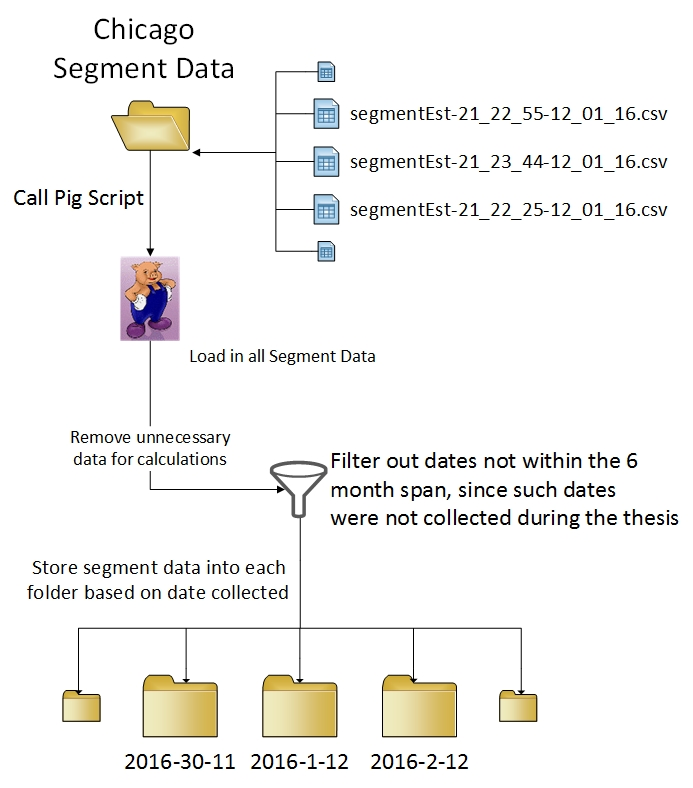
\includegraphics[scale=.4]{segmentFlow.jpg}
	\caption{\small Dataflow for cleaning and sorting the downloaded segment datasets}
	\label{fig:SegmentDataProcessing}
\end{figure}

\begin{figure}[H]
	\centering
	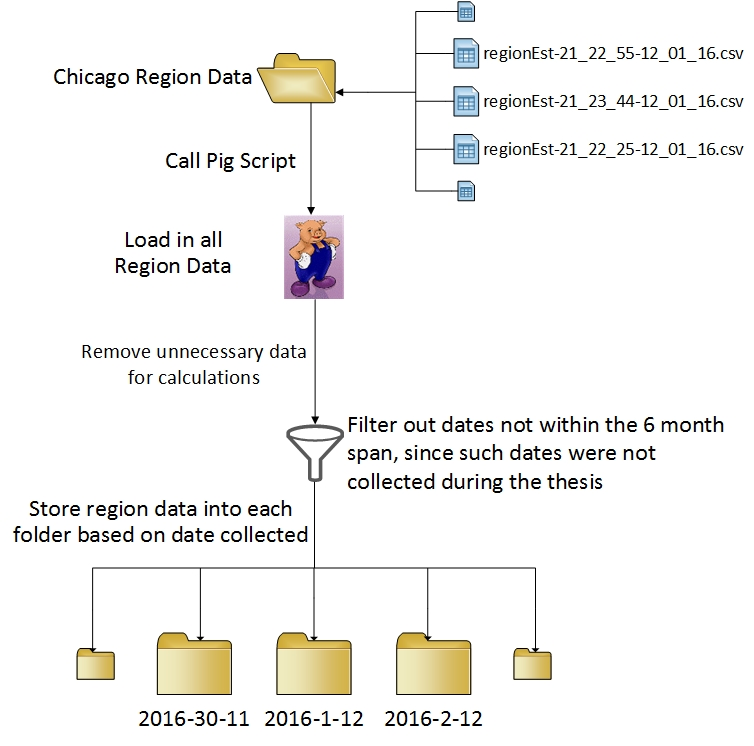
\includegraphics[scale=.4]{regionFlow.jpg}
	\caption{\small Dataflow for cleaning and sorting the downloaded region datasets}
	\label{fig:RegionDataProcessing}
\end{figure}

\subsubsection{Day Analysis}

\par Region data will take all the regions with the matching name and day to find the number of data points collected for a given day, number of times the speed is classified as high flow congestion, medium high flow congestion, medium flow congestion, light flow congestion, free flow congestion, the start time for the longest period of time of consecutive high flow and medium high flow congestion, and the end time for the high flow and medium high flow congestion, and the average speed during the time period. Algorithm \ref{alg:3} demonstrates the work of the reducer. All the counters are carried forward to be used as statistics and weights for determining if certain days are valuable to the analysis.

\begin{algorithm}
	\small
	\caption{\small Reducer from the MapReduce of analyizing each data for every region and outputting the data.}
	\label{alg:3}
	\begin{algorithmic}[1]
		\Procedure{reduce}{key, values}
		\State $ // Initialize\ values\ to\ zero $
		\State $ dc \gets 0 $ \Comment{dc = Data Count} 
		\State $ hfc \gets 0 $ \Comment{hfc = High Flow Count}
		\State $ mhfc \gets 0 $ \Comment{mhfc = Medium High Flow Count} 
		\State $ mfc \gets 0 $ \Comment{mfc = Medium Flow Count}
		\State $ lfc \gets 0 $ \Comment{lfc = Light Flow Count}
		\State $ ffc \gets 0 $ \Comment{ffc = Free Flow Count}
		\State $ sth = [] $ \Comment{List of speeds at time}
		\For{$ value: values $}
			\State $ dc++ $
			\State $ speed = value.speed $
			\State $ time = value.time $
			\State $ // Increment\ flow\ count\ based\ on\ speed $
			\If{$15 > speed >= 10  $}
				\State $ // mhfc\ value $
				\State $ sth[] \gets value.speed, value.time$
			\EndIf
			\If{$ 10 > speed >= 0 $}
				\State $ // hfc\ value $
				\State $ sth[] \gets value.speed, value.time $
			\EndIf
		\EndFor
		\State $ sth.sort() $ \Comment{Sort on time}
		\State $ ct = [] $ \Comment{Periods of congestions.}
		\State $ ch \gets NULL $ \Comment{New congestion holder}
		\State $ counter \gets 0 $ \Comment{Used for average speed}
		\For{$ i: sth  $}
			\State $ // Find\ consecutive\ times\ of\ congestion  $

			\If{$ ch == NULL $}
				\State $ startTime \gets NOW $
				\State $ endTime \gets NULL $
				\State $ avgSpd \gets i.speed $
				\State $ ch \gets startTime,endTime, avgSpd, (holders) $
				\State $ // Holders \gets dc,hfc,mhfc,mfc,lfc,ffc $
			\EndIf
			\If{$ ch\ NOT\ IsConsecutive(i)$}
				\State $ ch.endTime \gets NOW $
				\State $ ch.speed \gets  AVG(ch.speed, counter)$
				\State $ ct \gets ch $
				\State $ ch \gets NULL $ \Comment{New congestion holder}
				\State $ counter \gets 0 $ \Comment{Used for average speed}
			\EndIf
			\If{$ ch\ IsConsecutive( i )$}
				\State $ ch \gets (holder)++ $
				\State $ counter++ $
				\State $ ch.speed \gets ch.speed + i.speed $
			\EndIf
		\EndFor
		
		\State $ maxCongHolder \gets MAX(ch) $
		\State $ \Call{Store}{maxCongHolder} $
		\EndProcedure
	\end{algorithmic}
\end{algorithm}

\par Segment data will take all of the segments with the matching identifier and day to find the number of data points collected for a given day, the number of times the speed is classified as high flow congestions, medium flow congestion, free flow congestion, the start time for the longest period of time of consecutive high flow, and the end time for the longest period of time of consecutive high flow, and the number of negative speeds. The negative speeds were unique to segment data, showing that there has been no Chicago Traffic Authority buses through this segment, denoting that the segment has not been tracked. Algorithm \ref{alg:4} shows the work of the reducer. Algorithm \ref{alg:4} is similar to \ref{alg:3}, with the exception of different counters used. All the counters are carried forward to be used as statistics and weights for determining if certain days are valuable to the analysis.

\begin{algorithm}
	\small
	\caption{\small Reducer from the MapReduce of analyizing each data for every segment and outputting the data.}
	\label{alg:4}
	\begin{algorithmic}[1]
		\Procedure{reduce}{key, values}
		\State $ // Initialize\ values\ to\ zero $
		\State $ dc \gets 0 $ \Comment{dc = Data Count} 
		\State $ hfc \gets 0 $ \Comment{hfc = High Flow Count} 
		\State $ mfc \gets 0 $ \Comment{mfc = Medium Flow Count}
		\State $ ffc \gets 0 $ \Comment{ffc = Free Flow Count}
		\State $ ns \gets 0 $ \Comment{ns = Negative Speeds}
		\State $ sth = [] $ \Comment{List of speeds at time}
		\For{$ value: values $}
			\State $ dc++ $
			\State $ speed = value.speed $
			\State $ time = value.time $
			\State $ // Increment\ flow\ count\ based\ on\ speed $
			\If{$ 15 > speed >= 0 $}
				\State $ // hfc\ value $
				\State $ sth[] \gets value.speed, value.time $
			\EndIf
		\EndFor
		\State $ sth.sort() $ \Comment{Sort on time}
		\State $ ct = [] $ \Comment{Periods of congestions.}
		\State $ ch \gets NULL $ \Comment{New congestion holder}
		\State $ counter \gets 0 $ \Comment{Used for average speed}
		\For{$ i: sth  $}
			\State $ // Find\ consecutive\ times\ of\ congestion  $
			
			\If{$ ch == NULL $}
				\State $ startTime \gets NOW $
				\State $ endTime \gets NULL $
				\State $ avgSpd \gets i.speed $
				\State $ ch \gets startTime,endTime, avgSpd, (holders) $
				\State $ // Holders \gets dc,hfc,mfc,ffc,ns $
			\EndIf
			\If{$ ch\ NOT\ IsConsecutive(i)$}
				\State $ ch.endTime \gets NOW $
				\State $ ch.speed \gets  AVG(ch.speed, counter)$
				\State $ ct \gets ch $
				\State $ ch \gets NULL $ \Comment{New congestion holder}
				\State $ counter \gets 0 $ \Comment{Used for average speed}
			\EndIf
			\If{$ ch\ IsConsecutive( i )$}
				\State $ ch \gets (holder)++ $
				\State $ counter++ $
				\State $ ch.speed \gets ch.speed + i.speed $
			\EndIf
		\EndFor
		
		\State $ maxCongHolder \gets MAX(ch) $
		\State $ \Call{Store}{maxCongHolder} $
		\EndProcedure
	\end{algorithmic}
\end{algorithm}

\subsection{Grouping Analysis}
\label{sub:grpAnalysis}

\par After the MapReduce jobs \iffalse (Reducers Algorithm for Regions \ref{alg:3} and for Segments \ref{alg:4}) \fi complete, data for every day between the start date and the end date for segments and regions exist and a theme and rating for an advertisement exists for a segment and region. Using Pig, the traffic statistics and advertisement for a day and a given region and segment are joined together. 

\par After joining the advertisement data and the day analysis data, finding the best theme for a region and segment is be done using different time frames. By splitting up the data that fall on the same week of a year, month of a year, year, or keeping all the data together, there is a possibility of seeing a different outcome in determining a best theme during those time periods for each region and segment. 

\begin{algorithm}
	\small
	\caption{\small Reducer from the MapReduce of determining what is the best theme for a region and segment based on the time grouping. Different time groupings can be processed through this reducer. The difference between region and segment calculations are minute details in the code.}
	\label{alg:5}
	\begin{algorithmic}[1]
		\Procedure{reduce}{key, values}
		\State $ hcl \gets [] $ \Comment{hcl = High Congestion List}
		\State $ th \gets <> $ \Comment{th = Theme Holder}
		\State $ // Maps \gets theme -> totals, maxRating $
		\State $ td \gets 0 $ \Comment{td = Total Days}
		\For{$ v: values $}
			\State $ // v \gets sT, eT, avgSp, t, r, $
			\State $ // sT (Start\ Time), eT (End\ Time) $
			\State $ // avgSp (Average Speed), t (theme), r (Rating) $
			\State $ td++ $
			\If{$ \Call{Valid}{v.sT} AND \Call{Valid}{v.eT} $}
				\State $ hc \gets \Call{DumpAttr}{v} $
				\State $ hcl \gets hc $
				\State $ th \gets v.t $\Comment{Handles theme string}
				\State $ th \gets \Call{MAX}{th.maxRating, v.rating} $
			\EndIf
		\EndFor
		\If{$ hcl.size / td\  <\ .5\ OR\ hcl.empty\ ==\ TRUE$}
			\State $ \Call{RETURN}{Ignore} $
		\EndIf
		\State $ hcl \gets \Call{Overlap}{hcl} $ \Comment{Find overlap of times}
		\If{$ \Call{GetMaxSpeed}{hcl} < 25 $}
			\State $ \Call{Sort}{hcl} $
			\State $ max \gets \Call{Max}{hcl} $
			\State $ thm \gets max.theme $
			\State $ \Call{Return}{max, td, th.getRating(thm)} $
		\EndIf
		\State $ \Call{RETURN}{Ignore} $
		
		\EndProcedure
	\end{algorithmic}
\end{algorithm}

\par The reducer loops through the given values and gets times of high congestion that did not start and end at the exact same time. Using multiple maps, saving the maximum rating for a theme and the number of times the theme appears to easily update the values for a given theme. After looping through and finding all the high congestion times, various statistics that are calculated dynamically or provided from the day analysis factor in early if the time period and region are worthy of determining a theme. If low enough, the algorithm ignores the region for the time period. Otherwise, the algorithm attempts to combine all the congestion hour times to remove overlap for the given time period of a week, month, year, or of all time. Taking the largest congestion time, the segment or region, theme, and rating are returned for the given time period. 

\subsection{Querying the Results}

\par The traffic and advertisement sets for regions and segments are joined together then broken up by week, month, year, or all time to show the best advertisement for a given region or segment. Comparing the time break ups is not initially obvious, so the data needs to be aggregated to make comparisons easy between the different time periods. 

\par The results need to be presented so that a region and segment for a week, month, year, or all time have a similar layout. Using The \HadoopEcosystem\ and Hive, the resulting data from Algorithm \ref{alg:5} can be queried and aggregated. All data produced by the algorihm Section \ref{sub:grpAnalysis} are imported into a table structure in Hive. For the time periods of week, month, and year, the maximum rating for the longest time period an advertisement is shown over all time period break ups, presented the result in the table as one entity for a given week, month, and year.

\subsection{Code Repository}
\label{sub:github}

\par The code can be found at the following GitHub repository: \href{https://github.com/gateslm/CSSE-Senior-Thesis}{gateslm/CSSE-Senior-Thesis}

\section{Results and Discussion}

\par To see a subset of the results described before or a link to the full results, please refer to Appendix \ref{seg:segmentAnalysisData} and \ref{seg:regionAnalysisData}.

% \section{Discussion}

\par The outcome of region and segment results is as expected, however the result needs to be treated with caution as advertisement data, as the accuracy is not useful given the data is randomly generated. The results for any given region and segment does show that it is obvious that a billboard in a certain area would be highly ineffective, due to traffic flow in the area. This shows as a proof of concept that advertisement and traffic data can be aggregated together to provide evidence of advertisement do depend on traffic flow. 

\par Looking at how the data is grouped by week, month, year, or all together also shows the impact of a given length of an advertisement. Looking at the complete dataset, the algorithm found that some shorter time spans for a region and segment can be effective placements for billboards and the appropriate theme to use for that region/segment in a given time frame.  

\subsection{Region Result and Discussion}

\par The region results proved quite interesting. A large amount of advertisements and ratings stayed the same comparing between each time segments of month, year, and all time, but the week advertisement theme and rating would change. This can be associated with the algorithms found ties for advertisement lengths and ratings, and alphabetical order would be the determining factor for the resulting theme. 

\par Few regions had no themes and ratings that were all ignored for week, month, year, and all together. From the spreadsheet in the Appendix \ref{app:regionCTT}, a single row had month, year, and all together ignored. Had a week not be ignored does not seem out of place, since the length of congestion is long enough for a week, but not long enough to be congested for a large time period, month or year. A single week of the year could have had enough congestion to be considered for placing an advertisement. 

\subsection{Segment Result and Discussion}

\par The segment results had little variation. A large amount of advertisements and ratings stayed the same compared between each month, year, and all time, but the week advertisement theme and rating would change. This can be connected to the the fact that the algorithm would have ties of advertisement lengths and ratings, and alphabetical order would be the determining factor for the resulting theme. 

\par Many segments had no themes and ratings that were all ignored for week, month, year, and all together. By reading the description column on The \CityChicago\ Data Portal, many segments were no longer being recorded and had been left in the data sets.  From the spreadsheet in Appendix \ref{app:segmentCTT}, a vast amount of rows had month, year, and all together ignored. Had a week not be ignored does not seem out of place, since the length of congestion is long enough for a week, but not long enough to be congested for a large time period, month or year. A single week of the year could have had enough congestion to be considered for placing an advertisement. 

\section{Future Work}
\label{sec:futureWork}

\subsection{Data}

To substantially improve the accuracy of results would require different types of data. In this paper, all advertisement data is manually generated to be joined with region and segment traffic data. Advertisement data aimed at a specific city is not often available to the public due to privacy concerns and business practices. To get the success of billboards in a city, one would need to acquire the themes for the billboards, the time a given theme is presented on a billboard, and the location of all the billboards in a city. 

As described in Section \ref{sub:censusData}, census data can provide a variety of useful statistics that can factor in the theme of an advertisement much better than comparing the results of themes on a billboard. In a future extension of the thesis, census data could be incorporated into the regions and segments of Chicago or another city. By finding the percentage a zip code overlaps with a region or a segment, the influence of a certain type of advertisement could potentially be more influential than statistics based on studies of advertisement successes. Finding accurate listings of the zip codes in an easy to interpret file and access to current census data is needed. 

The amount of traffic data collected from The \CityChicago\ Data Portal was for the span of approximately 6 months, from September 18th, 2016 to February 23, 2017. To compare the success of aggregating the data based on week, month, year, or overall collection, a longer range of data would be needed to show relations. If data had been collected for over a year, then comparisons to similar times of a year could have been more obvious and highlighted patterns in the data. 

\subsection{Machine Learning}

An initial idea was to incorporate machine learning into the thesis  could not be used. The \HadoopEcosystem\ contained a tool that had a machine learning library, \textit{Spark}, could be used to apply filters over the data to aggregate the data a completely different way. Incorporating a type of machine learning into the data aggregation process could be ideal to show another potential overlap for \BigData\ to find patterns in the data. Due to time constraints and learning curves needed for software, the application of machine learning was not incorporated into this thesis. 

% \subsection{Alternative Big Data Analysis}


\cleardoublepage
\onecolumn
\section{Bibliography}

\bibliographystyle{plain}
\bibliography{bib}

\cleardoublepage
\twocolumn
\appendix
\section{Data Description}

\subsection{Chicago Traffic Tracker - Congestion Estimates by Segments}
\label{app:segmentCTT}

\underline{Column Names in Spreadsheet}
\begin{itemize}
	\item \textbf{SEGMENT\_ID}: Unique arbitrary number to represent each segment
	\item \textbf{STREET}: Street name of the traffic segment
	\item \textbf{DIRECTION}: Traffic flow direction for the segment
	\item \textbf{FROM\_STREET}: Start street for the segment in the direction of traffic flow
	\item \textbf{TO\_STREET}: End street for the segment in the direction of traffic flow
	\item \textbf{LENGTH}: Length of segment in miles
	\item \textbf{STREET\_HEADING}: Direction of the “STREET” from the origin point
	\item \textbf{START\_LATITUDE}, \textbf{START\_LONGITUDE}, \textbf{END\_LATITUDE}, \textbf{END\_LONGITUDE}: These four points represent the start and end points of the segment in the direction of traffic flow
	\item \textbf{CURRENT\_SPEED}: Real-time estimated speed in miles per hour
	\item \textbf{LAST\_UPDATED}: Date and time of update to spreadsheet
\end{itemize}

\subsection{Chicago Traffic Tracker - Congestion Estimates by Region}
\label{app:regionCTT}

\underline{Column Names in Spreadsheet}
\begin{itemize}
	\item \textbf{REGION}: Name of the region – made up of the names of the community areas within the region
	\item \textbf{REGION\_ID}: Unique arbitrary number to represent each region
	\item \textbf{WEST}: Lowest longitude values on the regions boundary
	\item \textbf{EAST}: Highest longitude values on the regions boundary
	\item \textbf{NORTH}: Highest latitude value on the regions boundary
	\item \textbf{SOUTH}: Lowest latitude value on the regions boundary
	\item \textbf{DESCRIPTION}: Describes the streets that demark the region’s boundary
	\item \textbf{CURRENT\_SPEED}: Real-time estimated congested level
	\item \textbf{LAST\_UPDATE}: Time stamp for the latest congestion estimation run.
\end{itemize}

\subsection{Advertisement Data Themes}
\label{app:adThemes}
\par Themes available to be selected when manually generating advertisements:
\begin{center}
\begin{tabular} { l c r}
	Automotive & Clothing & Educational \\ 
	Cellular Service & Technology & Medical \\
	Job & Recruitment & Housing \\
	Religious & Travel & Political \\
    Theater & Restaurant & Grocery \\ 
    Insurance & Mobile Devices & Toiletries \\
     Lawyer & Movie & Television \\
\end{tabular}
\end{center}

\onecolumn
\subsection{Region Analysis Data}
\label{seg:regionAnalysisData}
	\par Figure \ref{tab:subTableRegion} shows a subset of the data collected for regions. The subset of data is for doing tpython
	math.he algorithms over all the data without separation such as by weeks, months, or years. To see the full set of data for regions, refer to \href{https://docs.google.com/spreadsheets/d/1b-WJprSmBTCyujyXoT3wGxsx47cX5VVjYYHxUR9UrnU/edit?usp=sharing}{Google Drive Storage with all the data} separated by running the algorithm over weeks, months, or years.

\par NOTE: The values that have Ignore and negative numbers are place holders to denote where it was not relevant enough to place an advertisement. The different negative numbers are in place for debugging in case all output is a negative number for  a given region.

\begin{figure}[htbp]
	\centering
	% Table generated by Excel2LaTeX from sheet 'Sheet1'
    \begin{tabular}{|l|l|r|r|}
    	\hline
          & \multicolumn{3}{|c|}{All Data Result} \\
          \hline
    Region ID & Theme & \multicolumn{1}{|l|}{Theme Count} & \multicolumn{1}{|l|}{Rating} \\
    \hline
    Ashburn & Insurance & 48    & 9 \\
    Auburn Gresham-Chatham & Ignore & -1    & -1 \\
    Austin & Lawyer & 51    & 5 \\
    Beverly-Mt Greenwood-Morgan Park & Cellular Service & 47    & 10 \\
    Bridgeport-McKinley-Lower West & Clothing & 25    & 10 \\
    Chicago Loop & Travel & 54    & 9 \\
    Downtown Lakefront & Political & 16    & 9 \\
    Dunning-Portage-Belmont Cragn & Medical & 47    & 9 \\
    Edge Water-Uptown & Technology & 24    & 10 \\
    Far North West & Mobile Devices & 53    & 10 \\
    Fuller-Grand Blvd-Washington Park & Travel & 50    & 8 \\
    Hermosa-Logan Square & Mobile Devices & 28    & 9 \\
    Humboldt-Garfield Prk E/W & Ignore & -1    & -1 \\
    Hyde Park-Kenwood-Woodlawn & Mobile Devices & 31    & 9 \\
    Irving Park-Avondale-North Ctr & Housing & 45    & 10 \\
    Lawndale N/S & Religious & 54    & 6 \\
    Lawndale N/S & Religious & 54    & 6 \\
    Lincoln Park-Lake View & Mobile Devices & 38    & 10 \\
    Midway-Garfield Rdg-Clearing & Political & 24    & 9 \\
    Near North & Restaurant & 25    & 4 \\
    Near South-Douglas & Job   & 26    & 10 \\
    Near South-Douglas & Job   & 26    & 10 \\
    New City-Englewood-W Englewood & Ignore & -1    & -1 \\
    North Park-Albany-Linconl Sq & Movie & 30    & 10 \\
    North Park-Albany-Linconl Sq & Movie & 30    & 10 \\
    Riverdale-Hegewisch & Job   & 49    & 7 \\
    Riverdale-Hegewisch & Job   & 49    & 7 \\
    Riverdale-Hegewisch & Job   & 49    & 7 \\
    Rogers Park - West Ridge & Restaurant & 57    & 9 \\
    South Deering-East Side & Automotive & 37    & 8 \\
    South Shore-S Chicago-Avlon & Political & 32    & 10 \\
    South West Side & Ignore & -1    & -1 \\
    Washington Hts-Roseland-Pullman & Medical & 20    & 9 \\
    West Town-Near West & Ignore & -1    & -1 \\
    \hline
    \end{tabular}%


  \label{tab:subTableRegion}%
\caption{Subsection of Region data. The results were calculated using the described algorithms \ref{sec:algorithms} }
\end{figure}%

\clearpage

\subsection{Segment Analysis Data}
\label{seg:segmentAnalysisData}
\par Figure \ref{tab:tableSegmentSub} shows a subset of the data collected for segments. The subset of data is for doing the algorithms over all the data without separation such as by weeks, months, or years. To see the full set of data for segments, refer to \href{https://drive.google.com/open?id=1KnAJ8UV93-lr22eLf4HYYnbGWTztoq32c8p617_udOw}{Google Drive Storage with all the data} separated by running the algorithm over weeks, months, or years.


\par NOTE: The values that have Ignore and negative numbers are place holders to denote where it was not relevant enough to place an advertisement. The different negative numbers are in place for debugging in case all output is a negative number for  a given segment.

\begin{figure}[htbp]
	\centering
  % Table generated by Excel2LaTeX from sheet 'Sheet1'

    \begin{tabular}{|r|l|r|r|}
    	\hline
          & \multicolumn{3}{|c|}{All Data Result} \\
          \hline
    \multicolumn{1}{|l|}{Segment ID} & Theme & \multicolumn{1}{|l|}{Theme Count} & \multicolumn{1}{|l|}{Rating} \\
    \hline
    1     & Political & 40    & 5 \\
    2     & Clothing & 25    & 9 \\
    2     & Clothing & 25    & 9 \\
    3     & Technology & 12    & 10 \\
    4     & Movie & 19    & 9 \\
    4     & Movie & 19    & 9 \\
    5     & Ignore & -1    & -1 \\
    6     & Housing & 21    & 8 \\
    7     & Clothing & 3     & 10 \\
    8     & Mobile Devices & 33    & 8 \\
    9     & Job   & 16    & 10 \\
    10    & Mobile Devices & 46    & 8 \\
    11    & Toiletries & 52    & 7 \\
    12    & Mobile Devices & 14    & 9 \\
    13    & Television & 5     & 7 \\
    14    & Housing & 37    & 4 \\
    15    & Ignore & -1    & -1 \\
    16    & Ignore & -1    & -1 \\
    17    & Ignore & -1    & -1 \\
    19    & Ignore & -1    & -1 \\
    20    & Clothing & 3     & 9 \\
    21    & Ignore & -1    & -1 \\
    22    & Ignore & -1    & -1 \\
    23    & Ignore & -1    & -1 \\
    24    & Toiletries & 1     & 9 \\
    25    & Movie & 1     & 10 \\
    \hline
    \end{tabular}%


  \label{tab:tableSegmentSub}%
\caption{Subsection of Segment data. The results were calculated using the described algorithms \ref{sec:algorithms} }
\end{figure}%


\clearpage
\twocolumn

\end{document}